In this section two main theorems are stated.

\begin{thm}
	For a fixed $n$ there exists a $T$ which makes $(T, n)$ a good pair.
\end{thm}

\begin{thm}
	For a fixed $T$ and a large enough $n$, $(T, n)$ is not a good pair.
\end{thm}

The two theorems show that $(T, n)$ may possibly be good or bad when $T$ 
or $n$ changes. And we can see another fact by the proof then: the 
condition is better when a domain would not 'interfere' with
another domain.\newline

We prove the first theorem first as it is easier.

\begin{proof}[proof of Theorem 4.1]
	We just need to construct the $T$ for each $n$.
	
	Let $T$ be a rectangle of length $8n$ and width $2$, $A_k$ 
	be $(8k-4, 1)$(let the lower left corner of $T$ be the origin 
	point and establish coordinate system).
	
	To prove such an example meets the requirement, we need to prove
	that each $B$ changes at most an area of measure $8$ into green.
	
	Note that a point $B$ changes the points in at most three different 
	domains into green. So we just discuss by the number of domains $B$ changes.
	
	If $B$ changes two domains. We have two cases.\newline
	
	The first case: The area that $B$ changes is a trapezoid.
	
	\begin{center}
		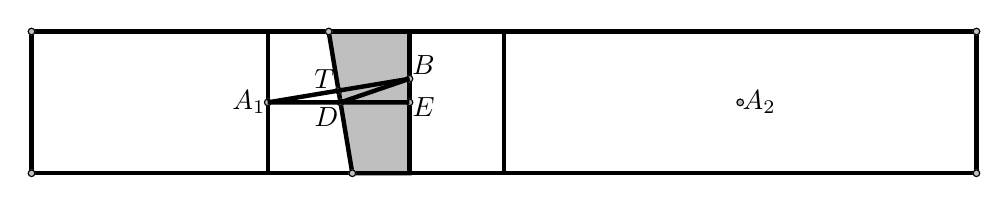
\begin{tikzpicture}[scale=0.6]
		\draw[ultra thick][black][fill=lightgray](8,0)--(8,3)--(6.29,3)
		--(6.79,0)--cycle;
		\draw[ultra thick][black](0,0)--(20,0)--(20,3)--(0,3)--cycle ;
		\draw[fill][lightgray](0,-0) circle [radius=0.07];
		\draw(0,-0) circle [radius=0.07];
		\draw[fill][lightgray](20,0) circle [radius=0.07];
		\draw(20,0) circle [radius=0.07];
		\draw[fill][lightgray](20,3) circle [radius=0.07];
		\draw(20,3) circle [radius=0.07];
		\draw[fill][lightgray](0,3) circle [radius=0.07];
		\draw(0,3) circle [radius=0.07];
		
		\draw[ultra thick][black](5,0)--(5,3);
		
		\draw[ultra thick][black](8,0)--(8,3);
		
		\draw[ultra thick][black](10,0)--(10,3);
		
		
		\draw[fill][lightgray](5,1.5) circle [radius=0.07];
		\draw(5,1.5) circle [radius=0.07];
		\node at (4.6,1.5){$A_1$};
		\draw[fill][lightgray](15,1.5) circle [radius=0.07];
		\draw(15,1.5) circle [radius=0.07];
		\node at (15.4,1.5){$A_2$};
		
		
		
		\draw[fill][lightgray](8,2) circle [radius=0.07];
		\draw(8,2) circle [radius=0.07];
		\node at (8.3,2.3){$B$};
		
		\draw[fill][lightgray](8,1.5) circle [radius=0.07];
		\draw(8,1.5) circle [radius=0.07];
		\node at (8.3,1.4){$E$};
		
		\draw[fill][lightgray](6.5,1.75) circle [radius=0.07];
		\draw(6.5,1.75) circle [radius=0.07];
		\node at (6.2,2){$T$};
		
		\draw[fill][lightgray](6.29,3) circle [radius=0.07];
		\draw(6.29,3) circle [radius=0.07];
		\draw[fill][lightgray](6.79,0) circle [radius=0.07];
		\draw(6.79,0) circle [radius=0.07];
		
		\draw[fill][lightgray](6.54,1.5) circle [radius=0.07];
		\draw(6.54,1.5) circle [radius=0.07];
		\node at (6.24,1.2){$D$};
		
		\draw[ultra thick][black](8,2)--(5,1.5)--(8,1.5);
		\draw[ultra thick][black](8,2)--(6.54,1.5);
		
		\end{tikzpicture}	
	\end{center}
	
	Label the points with letters as it shown in the picture above, 
	we figure out that $HI$ $LM$ are the perpendicular bisectors of 
	$A_1B$ and $A_2B$. We need to prove that $S_{HIML} \leq 4$. Note 
	that $|A_1D| =|BD| \geq |DE|$. Then we get $S_{HIGK} \leq S_{FHIJ}$. 
	Similarly we have that $S_{GKML} \leq S_{MLNO}$ and then 
	get the conclusion.\newline
	
	The second case: The area that $B$ changes is a triangle.
	
	\begin{center}
		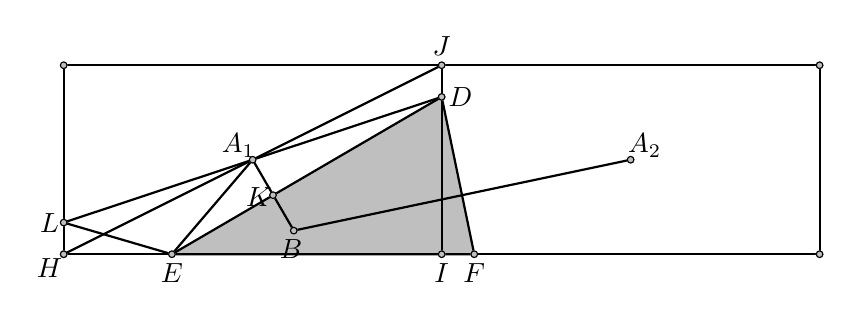
\begin{tikzpicture}[scale=0.6]
		\draw[thick][black][fill=lightgray](8,3.33)--(2.29,0)--(8.69,0)--cycle;
		
		\draw[thick][black](0,0)--(16,0)--(16,4)--(0,4)--cycle ;
		\draw[fill][lightgray](0,-0) circle [radius=0.07];
		\draw(0,-0) circle [radius=0.07];
		\draw[fill][lightgray](16,0) circle [radius=0.07];
		\draw(16,0) circle [radius=0.07];
		\draw[fill][lightgray](16,4) circle [radius=0.07];
		\draw(16,4) circle [radius=0.07];
		\draw[fill][lightgray](0,4) circle [radius=0.07];
		\draw(0,4) circle [radius=0.07];
		
		\draw[thick][black](8,0)--(8,4);
		
		\draw[thick][black](4,2)--(4.87,0.5)--(12,2);
		\draw[thick][black](8,4)--(0,0);
		\draw[thick][black](8,3.33)--(0,0.67)--(2.29,0)--(4,2);
		
		\draw[fill][lightgray](4,2) circle [radius=0.07];
		\draw(4,2) circle [radius=0.07];
		\node at (3.7,2.3){$A_1$};
		\draw[fill][lightgray](12,2) circle [radius=0.07];
		\draw(12,2) circle [radius=0.07];
		\node at (12.3,2.3){$A_2$};
		
		\draw[fill][lightgray](4.87,0.5) circle [radius=0.07];
		\draw(4.87,0.5) circle [radius=0.07];
		\node at (4.81,0.1){$B$};
		
		\draw[fill][lightgray](0,0) circle [radius=0.07];
		\draw(0,0) circle [radius=0.07];
		\node at (-0.3,-0.3){$H$};
		
		\draw[fill][lightgray](8,0) circle [radius=0.07];
		\draw(8,0) circle [radius=0.07];
		\node at (8,-0.4){$I$};
		
		\draw[fill][lightgray](8,4) circle [radius=0.07];
		\draw(8,4) circle [radius=0.07];
		\node at (8,4.4){$J$};
		
		\draw[fill][lightgray](0,0.67) circle [radius=0.07];
		\draw(0,0.67) circle [radius=0.07];
		\node at (-0.3,0.67){$L$};
		
		\draw[fill][lightgray](2.29,0) circle [radius=0.07];
		\draw(2.29,0) circle [radius=0.07];
		\node at (2.29,-0.4){$E$};
		
		\draw[fill][lightgray](4.43,1.25) circle [radius=0.07];
		\draw(4.43,1.25) circle [radius=0.07];
		\node at (4.13,1.2){$K$};
		
		\draw[fill][lightgray](8.69,0) circle [radius=0.07];
		\draw(8.69,0) circle [radius=0.07];
		\node at (8.69,-0.4){$F$};
		
		\draw[fill][lightgray](8,3.33) circle [radius=0.07];
		\draw(8,3.33) circle [radius=0.07];
		\node at (8.4,3.33){$D$};
		\end{tikzpicture}	
	\end{center}
	
	We may as well let the coordinate of the two origin points be 
	$(4, 1)$, $(12, 1)$. And the coordinate of $B$ be $(4+a, 1-b)$.
	
	\begin{equation}
	\begin{split}
	&S_{DIF} = \frac{1}{2}|DI||IF| = |DI| \times \frac{|DI|}{|k_{DF}|}
	\leq 2|DI||k_{BA_2}| = 2|DE|\frac{a}{\sqrt{a^2+b^2}}\frac{b}{8-a}\\ 
	\leq & |DE|\frac{b}{2}
	\leq |ED||KA_1|=2S_{EDA1}
	\leq S_{EDA1} + S_{LEA1} \\
	\leq & S_{EDA1}+S_{LHEA1} = S_{HEDJ}
	\end{split}
	\end{equation}
	
	So $S_{DEF}\leq S_{IJH}$.\newline
	
	If $B$ changes three domains.
	
	\begin{center}
		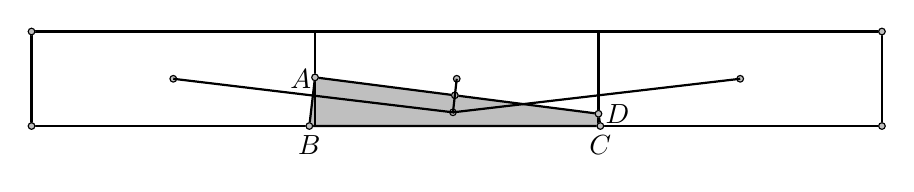
\begin{tikzpicture}[scale=0.6]
		
		\draw[thick][black][fill=lightgray](6,1.03)--(5.88,0)--
		(12.04,0)--(12,0.26)--cycle;
		\draw[thick][black](0,0)--(18,0)--(18,2)--(0,2)--cycle ;
		\draw[fill][lightgray](0,-0) circle [radius=0.07];
		\draw(0,-0) circle [radius=0.07];
		\draw[fill][lightgray](18,0) circle [radius=0.07];
		\draw(18,0) circle [radius=0.07];
		\draw[fill][lightgray](18,2) circle [radius=0.07];
		\draw(18,2) circle [radius=0.07];
		\draw[fill][lightgray](0,2) circle [radius=0.07];
		\draw(0,2) circle [radius=0.07];
		
		\draw[thick][black](6,0)--(6,2);
		
		\draw[thick][black](12,0)--(12,2);
		
		
		
		
		\draw[fill][lightgray](9,1) circle [radius=0.07];
		\draw(9,1) circle [radius=0.07];
		\draw[fill][lightgray](3,1) circle [radius=0.07];
		\draw(3,1) circle [radius=0.07];
		\draw[fill][lightgray](15,1) circle [radius=0.07];
		\draw(15,1) circle [radius=0.07];
		
		\draw[fill][lightgray](8.92,0.29) circle [radius=0.07];
		\draw(8.92,0.29) circle [radius=0.07];
		
		\draw[fill][lightgray](8.96,0.65) circle [radius=0.07];
		\draw(8.96,0.65) circle [radius=0.07];
		
		
		\draw[fill][lightgray](6,1.03) circle [radius=0.07];
		\draw(6,1.03) circle [radius=0.07];
		\node at (5.7,1){$A$};
		
		
		\draw[fill][lightgray](5.88,0) circle [radius=0.07];
		\draw(5.88,0) circle [radius=0.07];
		\node at (5.88,-0.4){$B$};
		
		
		\draw[fill][lightgray](12.04,0) circle [radius=0.07];
		\draw(12.04,0) circle [radius=0.07];
		\node at (12.04,-0.4){$C$};
		
		
		\draw[fill][lightgray](12,0.26) circle [radius=0.07];
		\draw(12,0.26) circle [radius=0.07];
		\node at (12.4,0.26){$D$};
		
		
		\draw[thick][black](9,1)--(8.92,0.29)--(3,1);
		\draw[thick][black](8.92,0.29)--(15,1);
		
		\end{tikzpicture}	
	\end{center}
	Let the coordinate of the three origin points be $(4, 1)$, $(12, 1)$, 
	$(20, 1)$. And coordinate of $B$ be $(12-a, 1-b)$, here $a$ and $b$ 
	are positive. We can calculate the area of $ABCD$.
	
	\begin{equation}
	\begin{split} &\frac{4b - 2b^2 - 2a^2}{b} + \frac{1}{2k_{AB}}
	(\frac{8a - a^2 + 2b - b^2}{2b})^2 + \frac{1}{2k_{CD}}
	(\frac{ - 8a - a^2 + 2b - b^2}{2b})^2 
	\\
	\leq& \frac{4b - 2b^2 - 2a^2}{b} + \frac{b}{7}(\frac{8a - a^2 + 2b
		- b^2}{2b})^2 + \frac{b}{7}(\frac{ - 8a - a^2 + 2b - b^2}{2b})^2
	\\
	\leq&4 - 2b + \frac{b}{7}(\frac{2b + 2b}{2b})^2 +
	\frac{b}{7}(\frac{2b}{2b})^2\\
	\leq& 4
	\end{split}
	\end{equation}
	
	In this inequality we use the conclusion that $4a \leq b$ and 
	$b \leq 1$. The first inequality can be proved by geometric 
	relationship $|BC|<|CA_2|$(or the B will just change two domains), 
	from the fact that $B$ changes three domains we can also get the 
	inequality that $a^2+b^2\geq 8a-2b$.
	
	This finish the proof of theorem4.1
\end{proof}

\begin{rem}
	In fact we haven't discussed all the cases, such as the case
	we discuss in the last of section3. But we know that the other cases 
	can be treated as a part of these three cases we have discussed.
\end{rem}

\begin{rem}
	It's clear that the length of small rectangles is not the best 
	constant here. The best constant of $length:width$ is around 2.
\end{rem}

Now it's time to go to our last main theorem, the main idea of proof 
is that when $n$ is big enough there must be a lot of quadrilateral 
and hexagonal domains. We need to find a contradiction in it.

At first we prove that there can't be quadrilaterals in most cases.

\begin{thm}
	If $A_1, A_2 ... A_n$ satisfy the condition and there is 
	a quadrilateral in $\iT_{Ai}$ , then the all the domains 
	must be like the case in theorem4.1 (a row of rectangles).
\end{thm}

\begin{proof}
	By lemma 5 the quadrilateral must be a parallelogram. 
	At first we prove that it must be a rectangle. For the origin 
	point of the quadrilateral $\iT_{A1}$, we notice that the symmetric 
	point of $A_1$ about the side of $\iT_{A1}$ which is not the bound 
	of T must be another origin point, we call it $A_2$, by lemma4 and 
	lemma5 we know that $\iT_{A_2}$ is also a quadrilateral. If $\iT_{A_1}$ 
	is not a rectangle, then two of its angle are obtuse angles, we select 
	the angle that one side is also the side of $\iT_{A_2}$ and label 
	it with letter $S$. Then we label other points like the picture.
	
	\begin{center}
		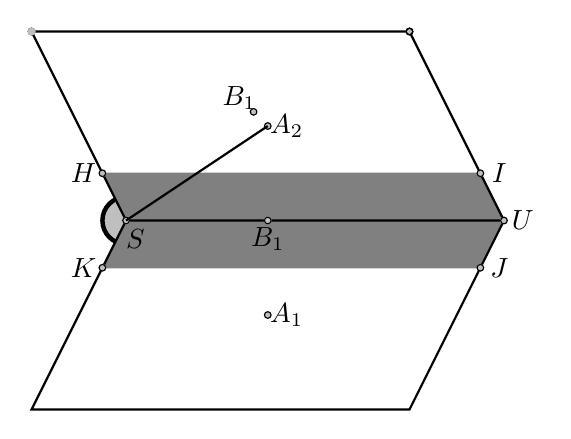
\begin{tikzpicture}[scale=0.6]
		\draw[ultra thick][fill=lightgray](0,0) circle [radius=0.5];
		
		\draw[fill][gray](8,0)--(7.5,1)--(-0.5,1)--(0,0)
		--(-0.5,-1)--(7.5,-1)--cycle;
		
		\draw[thick][black](0,0)--(8,0)--(6,4)--(-2,4)
		--(0,0)--(-2,-4)--(6,-4)--(8,0) ;
		\draw[fill][lightgray](0,-0) circle [radius=0.07];
		\draw(0,-0) circle [radius=0.07];
		\draw[fill][lightgray](8,0) circle [radius=0.07];
		\draw(8,0) circle [radius=0.07];
		\draw[fill][lightgray](6,4) circle [radius=0.07];
		\draw(6,4) circle [radius=0.07];
		\draw[fill][lightgray](-2,4) circle [radius=0.07];
		\draw(-2,4) circle [radius=0.07];
		\draw[fill][lightgray](-2,4) circle [radius=0.07];
		\draw(-2,4) circle [radius=0.07];
		\draw[fill][lightgray](-2,4) circle [radius=0.07];
		\draw(6,4) circle [radius=0.07];
		\draw[fill][lightgray](-2,4) circle [radius=0.07];
		\draw(6,4) circle [radius=0.07];
		
		\draw[fill][lightgray](3,2) circle [radius=0.07];
		\draw(3,2) circle [radius=0.07];
		\node at (3.4,2){$A_2$};
		
		\draw[fill][lightgray](3,-2) circle [radius=0.07];
		\draw(3,-2) circle [radius=0.07];
		\node at (3.4,-2){$A_1$};
		
		\draw[fill][lightgray](3,0) circle [radius=0.07];
		\draw(3,0) circle [radius=0.07];
		\node at (3,-0.4){$B_1$};
		
		\draw[fill][lightgray](2.7,2.3) circle [radius=0.07];
		\draw(2.7,2.3) circle [radius=0.07];
		\node at (2.4,2.6){$B_1$};
		
		\draw[fill][lightgray](7.5,1) circle [radius=0.07];
		\draw(7.5,1) circle [radius=0.07];
		\node at (7.9,1){$I$};
		
		\draw[fill][lightgray](7.5,-1) circle [radius=0.07];
		\draw(7.5,-1) circle [radius=0.07];
		\node at (7.9,-1){$J$};
		
		\draw[fill][lightgray](-0.5,1) circle [radius=0.07];
		\draw(-0.5,1) circle [radius=0.07];
		\node at (-0.9,1){$H$};
		
		\draw[fill][lightgray](-0.5,-1) circle [radius=0.07];
		\draw(-0.5,-1) circle [radius=0.07];
		\node at (-0.9,-1){$K$};	
		
		\draw[thick][black](3,2)--(0,0);
		\node at (8.4,0){$U$};
		\node at (0.2,-0.4){$S$};
		\end{tikzpicture}	
	\end{center}
	
	Call intersection of $US$ and $A_1A_2$ $B$. Here $HS = \frac{|ST|}{4}$ 
	then $B_1$ changes the black area into green. Consider the disk $D(S,r)$ 
	whose center is at $S$ with radius of $r = \frac{|SA_2-SB1|}{2}$. 
	The (purple) area of $D(S,r) \cap (\iT_{A1} \cup \iT_{A2})^c$ 
	is also turned to green by $B$ because for any point $T$ in $D(S,r)$ and
	another origin point $A$ we have that $|AT|\leq
	|AS|-\frac{|SA_2 - SB_1|}{2} \leq |SA_1| - \frac{|SA_2 - SB_1|}{2} 
	\leq |SB_1|$. So $B$ changes more than half (both gray and purple 
	part) of the quadrilateral. Then we use the trick we have used many 
	times to select other $B_i$ Then we get the contradiction.
	
	If $\iT_{A_1}$ is a rectangle, using the trick we used in section3 
	we know that all domains are rectangles and they make up a table. 
	Using the proof in section3 again we can know that the table only 
	have one row(or one column) thus we get the conclusion.
\end{proof}

So only if $T$ is a rectangle then there could be quadrilateral 
in $\iT_{A_1}, \iT_{A_2} ... \iT_{A_n}$. But when $T$ is a rectangle 
and $n$ becomes big enough it becomes a case in section3 which turns 
out to be bad. 

The we prove that there would be a lot of hexagons. Euler's Formula 
: $V-E+F=1$ to prove this thing.

\begin{thm}
	We divide a polygon $T$ into small polygons with even edges. 
	If there aren't quadrilaterals, the numbers of `points on edges', 
	`the polygons which has more than eight edges', `the points in $T$ 
	who is the endpoint of more than four lines' can be controlled 
	by a constant $c$ only depended on $T$.
\end{thm}

\begin{rem}
	By lemma 6 $T_i$ must be polygons (we even know it's a centrally 
	symmetric polygon), and all the numbers of edges of polygons must
	be even. So we naturally consider theorem4.4. 
\end{rem}

\begin{proof}
	Let $n$ be the number of edges of $T$ , $p$ be the number of points
	on edges, $r$ be the number of points in $T$, $h$ be the number of 
	hexagons, $t$ be the number of polygons which has more than seven 
	edges, $l$ be the number of lines in $T$, $f$ be the the number of 
	the points in $T$ who is the endpoint of more than four lines.
	
	Then we have
	
	\[
	\begin{cases}
	n - 2 + p + 2r \geq 4h + 6t\\
	h + t + p + r - l - p = 1 \\
	l \geq \frac{p + 3r + f}{2}
	\end{cases}
	\]
	
	The first inequality is gotten by calculating degrees, 
	the second one comes from  Euler's Formula and the third one 
	is because every point inside $T$ has at least 3 lines from it 
	and every point on edges has at least one.
	
	solve the inequalities system we get that $n - 6 \geq p + 2t + 2f$ and
	we get the conclusion.
\end{proof}	

This theorem gives out a way leading to our goal. It tells us 
that there are enough hexagons which are not on the edges. It's 
interesting that a hexagon will not cause contradiction directly 
but when a hexagon is surrounded by others hexagons we can get 
contradiction.


By theorem4.4 we know that if $n$ is big enough we can select a 
lot of adjacent hexagons, every of which is surrounded by other 
six hexagons and each vertex of the original hexagon is just the
vertex of three domains.

Consider such a hexagon:

\begin{thm}
	Such a hexagon must be a diagonal parallel hexagon.
\end{thm}	 

We give out the definition of parallel hexagon then.

\begin{defn}
	A diagonal parallel hexagon is a hexagon that each main 
	diagonal is parallel to the opposite.
\end{defn}


\begin{center}
	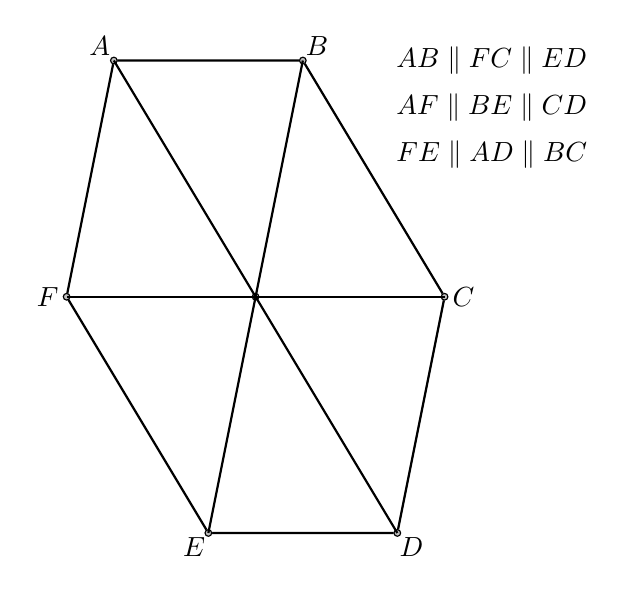
\begin{tikzpicture}[scale=0.6]
	
	\draw[thick][black](4,0)--(1,5)--(-3,5)--(-4,0)--(-1,-5)--(3,-5)--cycle ;
	\draw[fill][lightgray](4,-0) circle [radius=0.07];
	\draw(4,-0) circle [radius=0.07];
	\draw[fill][lightgray](1,5) circle [radius=0.07];
	\draw(1,5) circle [radius=0.07];
	\draw[fill][lightgray](-3,5) circle [radius=0.07];
	\draw(-3,5) circle [radius=0.07];
	\draw[fill][lightgray](-4,0) circle [radius=0.07];
	\draw(-4,0) circle [radius=0.07];
	\draw[fill][lightgray](-1,-5) circle [radius=0.07];
	\draw(-1,-5) circle [radius=0.07];
	\draw[fill][lightgray](3,-5) circle [radius=0.07];
	\draw(3,-5) circle [radius=0.07];
	\draw[fill][lightgray](0,0) circle [radius=0.07];
	\draw(0,0) circle [radius=0.07];
	\draw[thick][black](4,0)--(-4,0);
	\draw[thick][black](1,5)--(-1,-5);
	\draw[thick][black](-3,5)--(3,-5);
	
	\node at (-3.3,5.3){$A$};
	\node at (1.3,5.3){$B$};
	\node at (4.4,0){$C$};
	\node at (3.3,-5.3){$D$};
	\node at (-1.3,-5.3){$E$};
	\node at (-4.4,0){$F$};
	
	\node at (5,5){$AB\parallel FC\parallel ED$};
	\node at (5,4){$AF\parallel BE\parallel CD$};
	\node at (5,3){$FE\parallel AD\parallel BC$};	
	\end{tikzpicture}	
\end{center}

Now we give out the proof, the idea is based on translating $B$ 
a little distance from $A$, because the calculating of areas is a 
bit complicated, we use different colors to sign different domain 
for convenience. We clarify our notation, let $\T$ be any function such that $\lim_{\epsilon \to 0}\frac{\T(\epsilon)}{\epsilon} = 1$, and
$o(\epsilon)$ be higher order infinitesimal of $\epsilon$.


\begin{center}
	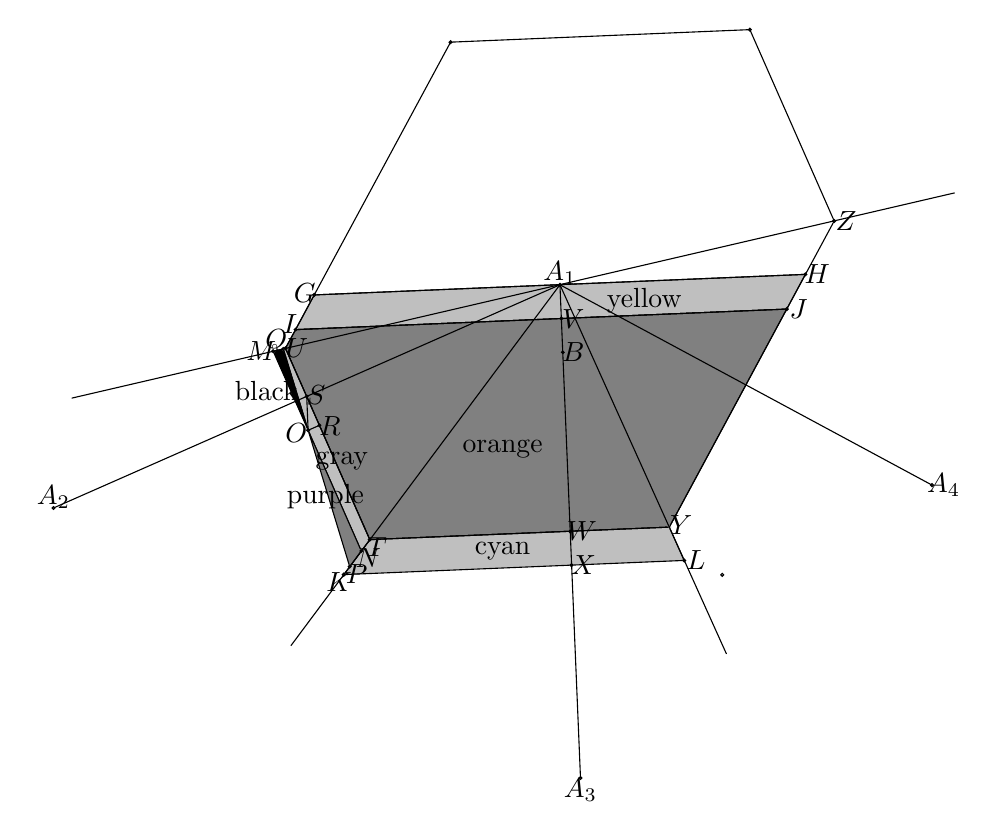
\begin{tikzpicture}[scale=0.3]
	
	\draw[black][fill=lightgray](-13.97,6.55)--(6.82,7.42)--(6.03,5.95)--(-14.76,5.08)--cycle;
	\draw[black][fill=gray](-14.76,5.08)--(6.03,5.95)--(1.06,-3.28)--(-11.62,-3.81)--(-15.19,4.29)--cycle;
	\draw[black][fill=lightgray](-11.62,-3.81)--(1.06,-3.28)--(1.69,-4.69)--(-12.72,-5.29)--cycle;
	\draw[black][fill=lightgray](-15.28,4.26)--(-15.19,4.29)--(-11.62,-3.81)--(-11.98,-4.29)--(-14.23,0.82)--cycle;
	\draw[black][fill=gray](-14.23,0.82)--(-11.98,-4.29)--(-12.47,-4.95)--cycle;
	\draw[black][fill=black](-15.28,4.26)--(-14.23,0.82)--(-15.71,4.17)--cycle;
	
	
	\draw[fill][lightgray](-25.01,-2.47) circle [radius=0.06];
	\draw(-25.01,-2.47) circle [radius=0.06];
	\node at (-25.01,-2){$A_2$}; 
	\draw[fill][lightgray](-15.71,4.17) circle [radius=0.06];
	\draw(-15.71,4.17) circle [radius=0.06];
	\node at (-16.21,4.17){$M$};
	\draw[fill][lightgray](-15.28,4.26) circle [radius=0.06];
	\draw(-15.28,4.26) circle [radius=0.06];	
	\node at (-15.58,4.56){$Q$};
	\draw[fill][lightgray](-13.97,6.55) circle [radius=0.06];
	\draw(-13.97,6.55) circle [radius=0.06];
	\node at (-14.37,6.65){$G$};
	\draw[fill][lightgray](-14.76,5.08) circle [radius=0.06];
	\draw(-14.76,5.08) circle [radius=0.06];
	\node at (-15,5.3){$I$};
	\draw[fill][lightgray](-15.19,4.29) circle [radius=0.06];
	\draw(-15.19,4.29) circle [radius=0.06];
	\node at (-14.7,4.29){$U$};
	\draw[fill][lightgray](-14.29,2.26) circle [radius=0.06];
	\draw(-14.29,2.26) circle [radius=0.06];
	\node at (-13.89,2.3){$S$};
	\draw[fill][lightgray](-14.23,0.82) circle [radius=0.06];
	\draw(-14.23,0.82) circle [radius=0.06];
	\node at (-14.73,0.7){$O$};
	\draw[fill][lightgray](-13.75,1.03) circle [radius=0.06];
	\draw(-13.75,1.03) circle [radius=0.06];
	\node at (-13.3,1){$R$};
	\draw[fill][lightgray](-12.72,-5.29) circle [radius=0.06];
	\draw(-12.72,-5.29) circle [radius=0.06];
	\node at (-12.92,-5.593){$K$};
	\draw[fill][lightgray](-12.47,-4.95) circle [radius=0.06];
	\draw(-12.47,-4.95) circle [radius=0.06];
	\node at (-12.17,-5.25){$P$};
	\draw[fill][lightgray](-11.98,-4.29) circle [radius=0.06];
	\draw(-11.98,-4.29) circle [radius=0.06];
	\node at ((-11.68,-4.59){$N$};
	\draw[fill][lightgray](-11.62,-3.81) circle [radius=0.06];
	\draw(-11.62,-3.81) circle [radius=0.06];
	\node at (-11.32,-4.11){$T$};
	\draw[fill][lightgray](-3.57,6.98) circle [radius=0.06];
	\draw(-3.57,6.98) circle [radius=0.06];
	\node at (-3.57,7.48){$A_1$};
	\draw[fill][lightgray](-3.51,5.55) circle [radius=0.06];
	\draw(-3.51,5.55) circle [radius=0.06];
	\node at (-3.01,5.55){$V$};
	\draw[fill][lightgray](-3.45,4.12) circle [radius=0.06];
	\draw(-3.45,4.12) circle [radius=0.06];
	\node at (-3,4.12){$B$};
	\draw[fill][lightgray](-3.14,-3.46) circle [radius=0.06];
	\draw(-3.14,-3.46) circle [radius=0.06];
	\node at (-2.64,-3.46){$W$};
	\draw[fill][lightgray](-3.08,-4.89) circle [radius=0.06];
	\draw(-3.08,-4.89) circle [radius=0.06];
	\node at (-2.58,-4.89){$X$};
	\draw[fill][lightgray](1.69,-4.69) circle [radius=0.06];
	\draw(1.69,-4.69) circle [radius=0.06];
	\node at (2.19,-4.69){$L$};
	\draw[fill][lightgray](1.06,-3.28) circle [radius=0.06];
	\draw(3.3,-5.3) circle [radius=0.06];
	\node at (1.56,-3.2){$Y$};
	\draw[fill][lightgray](6.03,5.95) circle [radius=0.06];
	\draw(6.03,5.95) circle [radius=0.06];
	\node at (6.53,5.95){$J$};
	\draw[fill][lightgray](6.82,7.42) circle [radius=0.06];
	\draw(6.82,7.42) circle [radius=0.06];
	\node at (7.32,7.42){$H$};
	\draw[fill][lightgray](8.04,9.68) circle [radius=0.06];
	\draw(8.04,9.68) circle [radius=0.06];
	\node at (8.54,9.68){$Z$};
	\draw[fill][lightgray](12.18,-1.5) circle [radius=0.06];
	\draw(12.18,-1.5) circle [radius=0.06];
	\node at (12.68,-1.5){$A_4$};
	\draw[fill][lightgray](-8.2,17.25) circle [radius=0.06];
	\draw(-8.2,17.25)circle [radius=0.06];
	\draw[fill][lightgray](4.47,17.78) circle [radius=0.06];
	\draw(4.47,17.78) circle [radius=0.06];
	\draw[fill][lightgray](-2.7,-13.9) circle [radius=0.06];
	\draw(-2.7,-13.9) circle [radius=0.06];	
	\node at (-2.7,-14.4){$A_3$};
	
	
	
	
	\draw[black](-8.2,17.25)--(4.47,17.78)--(8.04,9.68)--(1.06,-3.28)--(-11.62,-3.81)--(-15.19,4.29)--cycle;
	\draw[black](-13.97,6.55)--(6.82,7.42);
	\draw[black](-14.76,5.08)--(6.03,5.95);
	\draw[black](13.14,10.87)--(-24.24,2.18);
	\draw[black](-3.57,6.98)--(-25.01,-2.47);
	\draw[black](-3.57,6.98)--(-14.96,-8.3);
	\draw[black](-3.57,6.98)--(-2.7,-13.9);
	\draw[black](-3.57,6.98)--(3.48,-8.65);
	\draw[black](-3.57,6.98)--(12.18,-1.5);
	\draw[black](-14.29,2.26)--(-14.23,0.82)--(-13.75,1.03);
	
	
	\node at (0,6.3){yellow};
	\node at (-6,0){orange};
	\node at (-6,-4.3){cyan};
	\node at (-12.8,-0.5){gray};
	\node at (-13.5,-2){purple};
	\node at (-16,2.5){black};
	\end{tikzpicture}
\end{center}

\begin{proof}
	At first we tell the construction of points in the picture.
	We translate $B$ a infinitesimal $\epsilon$ from $A$ on the line $AW$
	which is the vertical line from $A$ to $ST$. $A_2$, $A_3$ and $A_4$ are
	the symmetric point of $A$ about $UT$, $TS$ and $SR$. $IJ$, $MN$ and 
	$KL$ are perpendicular bisectors of$A_1B$, $A_1A_2$ and $BA_3$. 
	The intersection of $BA_2$ and $MN$ are $O$, $PQ$ is the lines which 
	vertical to $BA_2$ and passed $O$.
	
	$B$ changes the orange, black, gray, purple and the symmetrical part
	of gray and purple(call it $D$) into its own domain. 
	
	What we want to prove now is that $S_{cyan} + S_{gray} +
	S_{purple} + S_{D} - S_{yellow} = c\T(\epsilon) $ 
	Here $c\geq0$ and is $0$ iff the
	hexagon is a parallel hexagon.
	
	Notice that $S_{yellow} = \frac{|GH|}{2}\T(\epsilon)$, $S_{cyan} = \frac{|TY|}{2}\T(\epsilon)$ because we have that that $|A_1V| = |WX| = \frac{\epsilon}{2}$
	
	Now calculate $S_{gray}+S_{purple}$. Let $f_{UT} = |TS| - |SU|$ 
	and $\theta$ be $\pi - \angle UTS$
	
	At first we notice that 
	
	\begin{equation}
	\begin{split}
	&S_{gray} + S_{black}\\
	=&|UT|(|OR| + o(|OR))\\
	=&|UT|(|SO||\cos \angle SOR + o(SO)|\\
	=&|UT|\cos\theta \frac{\T(\epsilon)}{2}
	\end{split}
	\end{equation}
	
	and	
	
	\begin{equation}
	\begin{split}
	&S_{purple} - S_{black}\\
	=&\T(\frac{1}{2}|NO^2 - MO^2||\sin\angle PON|)\\
	=&\T(\frac{1}{2}|TS^2 - SU^2|\sin \angle A_1A_2B)\\
	=&\T(d_{UT}|UT|\epsilon\frac{\sin \angle A_2A_1B}{A_1A_2})
	\end{split}
	\end{equation}
	
	So $B$ changes the domain of area.
	($\theta'$ means the $\pi - \angle RST$)
	\begin{equation}
	\begin{split}
	&\frac{S_{hexagon}}{2} + |UT|\cos\theta \frac{\T(\epsilon)}{2} + \T(d_{UT}|UT|\epsilon\frac{\sin \angle A_2A_1B}{A_1A_2} + 
	|RS|\cos\theta' \frac{\T(\epsilon)}{2}\\
	-& \T(d_{SR}|SR|\epsilon\frac{\sin \angle A_4A_1B}{A_4A_2}) - \frac{|GH|}{2}\T(\epsilon) + 
	\frac{|TS|}{2}\T(\epsilon)
	\\
	= & \frac{S_{hexagon}}{2} + \T((\epsilon)
	(\frac{1}{2}|UT|\cos\theta )
	+\frac{1}{2}|RS|\cos\theta' +(f_{UT}|UT|\frac{\sin 
		\angle A_2A_1B}{A_1A_2})\\
	- &(f_{SR}|SR|\frac{\sin \angle A_4A_1B}{A_4A_2}) + 
	\frac{|TS|}{2} - \frac{|GH|}{2})
	\end{split}
	\end{equation}
	
	It's the case that $B$ moves a little distance $\epsilon$ 
	on the vertical line from $A$ to $ST$, we let this $B$ be $B_1$. 
	Similarly if $B$ moves $\epsilon$ on the perpendicular lines to 
	other edges and we calculate the average of them we get that $B$ 
	changes the domain of area 
	
	\[ \frac{S_{hexagon}}{2} + \frac{1}{6} \T(\epsilon)(\frac{1}{2}\sum _{cyc}(|UT|\cos\theta+|RS|\cos\theta'+|TS|-|GH|)) \]
	
	Here cyc means sum interchangeably.
	
	We notice that$|UT|\cos\theta + |RS|\cos\theta' + |TS|\geq|GH|$ 
	and the equation established iff $GH \backslash \backslash TS$. 
	We can prove this by geometric relationship. There are three cases.
	First of two are:
	
	\begin{center}
		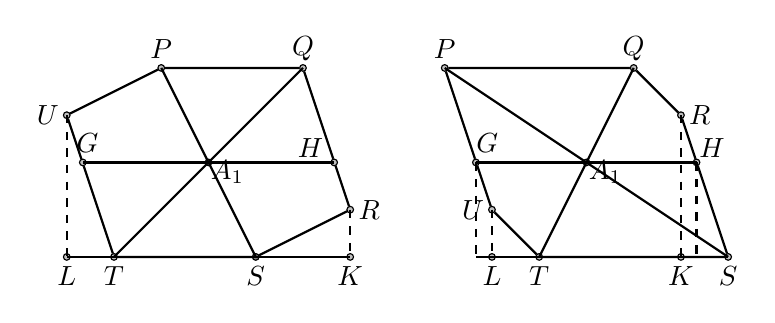
\begin{tikzpicture}[scale=0.6]
		
		\draw[thick][black](3,-1)--(1,-2)--(-2,-2)--(-3,1)
		--(-1,2)--(2,2)--cycle ;
		\draw[fill][lightgray](3,-1) circle [radius=0.07];
		\draw(3,-1)circle [radius=0.07];
		\node at (3.4,-1){$R$};
		\draw[fill][gray](1,-2) circle [radius=0.07];
		\draw(1,-2) circle [radius=0.07];
		\node at (1,-2.4){$S$};
		\draw[fill][lightgray](-2,-2) circle [radius=0.07];
		\draw(-2,-2) circle [radius=0.07];
		\node at (-2,-2.4){$T$};
		\draw[fill][lightgray](-3,1) circle [radius=0.07];
		\draw(-3,1) circle [radius=0.07];
		\node at (-3.4,1){$U$};
		\draw[fill][lightgray](-1,2) circle [radius=0.07];
		\draw(-1,2) circle [radius=0.07];
		\node at (-1,2.4){$P$};
		\draw[fill][lightgray](2,2) circle [radius=0.07];
		\draw(2,2) circle [radius=0.07];
		\node at (2,2.4){$Q$};
		\draw[fill][lightgray](0,0) circle [radius=0.07];
		\draw(0,0) circle [radius=0.07];
		\node at (0.4,-0.2){$A_1$};
		\draw[fill][lightgray](2.66,0) circle [radius=0.07];
		\draw(2.66,0) circle [radius=0.07];
		\node at (2.16,0.3){$H$};
		\draw[fill][lightgray](-2.66,0) circle [radius=0.07];
		\draw(-2.66,0) circle [radius=0.07];
		\node at (-2.56,0.4){$G$};
		\draw[fill][lightgray](3,-2) circle [radius=0.07];
		\draw(3,-2) circle [radius=0.07];
		\node at (3,-2.4){$K$};
		\draw[fill][lightgray](-3,-2) circle [radius=0.07];
		\draw(-3,-2) circle [radius=0.07];
		\node at (-3,-2.4){$L$};
		
		\draw[thick][black](2,2)--(-2,-2);
		\draw[thick][black](1,-2)--(-1,2);
		\draw[thick][black](2.66,0)--(-2.66,0);
		\draw[dashed, thick][black](3,-1)--(3,-2);
		\draw[dashed, thick][black](-3,1)--(-3,-2);
		\draw[thick][black](-3,-2)--(3,-2);
		
		\draw[thick][black](10,1)--(11,-2)--(7,-2)--(6,-1)
		--(5,2)--(9,2)--cycle ;
		\draw[fill][lightgray](10,1) circle [radius=0.07];
		\draw(10,1)circle [radius=0.07];
		\node at (10.4,1){$R$};
		\draw[fill][lightgray](11,-2) circle [radius=0.07];
		\draw(11,-2)circle [radius=0.07];
		\node at (11,-2.4){$S$};
		\draw[fill][lightgray](7,-2) circle [radius=0.07];
		\draw(7,-2) circle [radius=0.07];
		\node at (7,-2.4){$T$};
		\draw[fill][lightgray](6,-1) circle [radius=0.07];
		\draw(6,-1) circle [radius=0.07];
		\node at (5.6,-1){$U$};
		\draw[fill][lightgray](5,2) circle [radius=0.07];
		\draw(5,2) circle [radius=0.07];
		\node at (5,2.4){$P$};
		\draw[fill][lightgray](9,2) circle [radius=0.07];
		\draw(9,2) circle [radius=0.07];
		\node at (9,2.4){$Q$};
		\draw[fill][lightgray](8,0) circle [radius=0.07];
		\draw(8,0) circle [radius=0.07];
		\node at (8.4,-0.2){$A_1$};
		\draw[fill][lightgray](10.33,0) circle [radius=0.07];
		\draw(10.33,0) circle [radius=0.07];
		\node at (10.66,0.3){$H$};
		\draw[fill][lightgray](5.66,0) circle [radius=0.07];
		\draw(5.66,0) circle [radius=0.07];
		\node at (5.9,0.4){$G$};
		\draw[fill][lightgray](10,-2) circle [radius=0.07];
		\draw(10,-2) circle [radius=0.07];
		\node at (10,-2.4){$K$};
		\draw[fill][lightgray](6,-2) circle [radius=0.07];
		\draw(6,-2) circle [radius=0.07];
		\node at (6,-2.4){$L$};
		
		\draw[thick][black](5.66,0)--(10.33,0);
		\draw[thick][black](9,2)--(7,-2);
		\draw[thick][black](11,-2)--(5,2);
		\draw[dashed, thick][black](6,-1)--(6,-2);
		\draw[dashed, thick][black](10,1)--(10,-2);
		\draw[thick][black](5.66,-2)--(11,-2);
		\draw[dashed, thick][black](5.66,0)--(5.66,-2);
		\draw[dashed, thick][black](10.33,0)--(10.33,-2);
		\end{tikzpicture}	
	\end{center}
	
	For the first case we know that 
	\[ |UT|\cos\theta+|RS|\cos\theta' + |TS| \geq |JT| + |TS| + |SK|
	\geq|TS| \]
	
	For the second case we know that
	\[ LHS\geq|JT| + |TS| + |SK| = |JW| + |WS|\geq |JW| + 
	|WK| = |TS| \]
	
	So $|UT|\cos\theta+|RS|\cos\theta'+|TS|-|GH|\geq 0$.
	
	If the equation didn't establish, then we can always find a $B$ 
	in the hexagon and $B$ changes more than half area of the hexagon 
	into its own domain.And then use the tricks we have used many 
	times to select other $B_i$. 
	So the equation all established.
	
	There is one case left: when $UT\perp TS$, the projection of $GH$ 
	is the same as $UR$. In that case, we can change the direction of $B$ 
	moved from $A$ to get contradiction. 
\end{proof}

When we have such a strong conclusion, we can select three adjacent 
hexagons and calculate the angles to get further conclusion.

\begin{thm}
	If 3 hexagons are adjacent, they are all regular hexagons.
\end{thm}

\begin{center}
	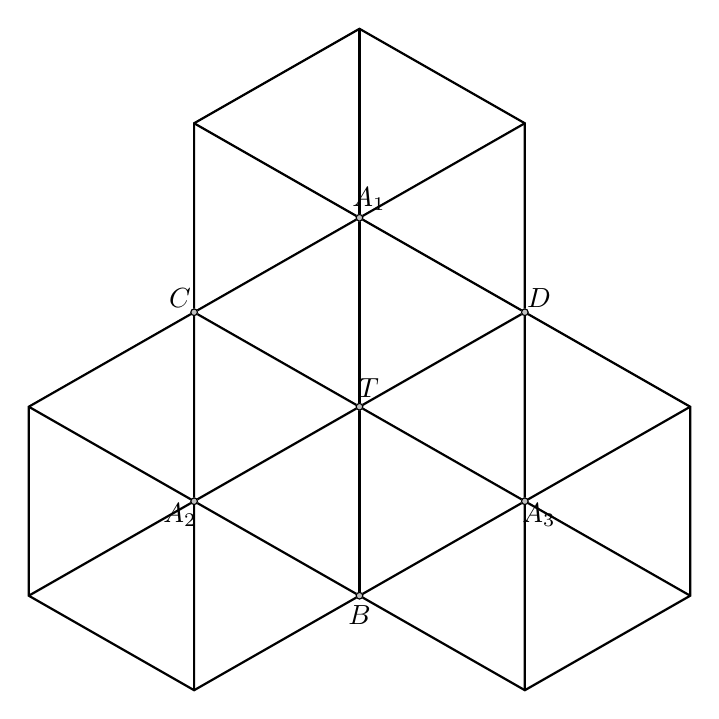
\begin{tikzpicture}[scale=0.6]
	
	
	\draw[thick][black](0,8)--(3.5,6)--(3.5,2)--(7,0)--(7,-4
	)--(3.5,-6)--(0,-4)--(-3.5,-6)--(-7,-4)--(-7,0)--(-3.5,2)
	--(-3.5,6)--cycle ;
	\draw[thick][black](0,4)--(3.5,2)--(3.5,-2)--(0,-4)--
	(-3.5,-2)--(-3.5,2)--cycle ;
	\draw[thick][black](0,8)--(0,4)--(0,0)--(0,-4) ;	
	\draw[thick][black](-7,-4)--(-3.5,-2)--(0,0)--(3.5,2);
	\draw[thick][black](7,-4)--(3.5,-2)--(0,0)--(-3.5,2);
	\draw[thick][black](-3.5,6)--(0,4)--(3.5,6);
	\draw[thick][black](-7,0)--(-3.5,-2)--(-3.5,-6);
	\draw[thick][black](7,0)--(3.5,-2)--(3.5,-6);
	
	\draw[fill][lightgray](0,-0) circle [radius=0.07];
	\draw(0,-0) circle [radius=0.07];
	\node at (0.2,0.4){$T$};
	\draw[fill][lightgray](0,4) circle [radius=0.07];
	\draw(0,4) circle [radius=0.07];
	\node at (0.2,4.4){$A_1$};
	\draw[fill][lightgray](-3.5,2) circle [radius=0.07];
	\draw(-3.5,2) circle [radius=0.07];
	\node at (-3.8,2.3){$C$};
	\draw[fill][lightgray](-3.5,-2) circle [radius=0.07];
	\draw(-3.5,-2) circle [radius=0.07];
	\node at (-3.8,-2.3){$A_2$};
	\draw[fill][lightgray](0,-4) circle [radius=0.07];
	\draw(0,-4) circle [radius=0.07];
	\node at (0,-4.4){$B$};
	\draw[fill][lightgray](3.5,-2) circle [radius=0.07];
	\draw(3.5,-2) circle [radius=0.07];
	\node at (3.8,-2.3){$A_3$};
	\draw[fill][lightgray](3.5,2) circle [radius=0.07];
	\draw(3.5,2) circle [radius=0.07];
	\node at (3.8,2.3){$D$};
	\end{tikzpicture}	
\end{center}


\begin{proof}
	We just need to calculate angles. In the equation we use the facts 
	that $A_1BTC$, $A_3DTB$ and $A_2DTC$ are parallelograms, 
	$A_1$ and $A_2$ and $A_3$ are symmetric points about 
	$TC$, $TD$, and $TB$.
	
	\begin{equation}
	\begin{split}
	&\angle TA_3B = \angle DTA_3 = \pi - \angle CTB = \angle TBA_1
	\end{split} 
	\end{equation}
	
	Similarly we have that $\angle TA_1B = \angle TBA_3$. Then we 
	get that $\angle BTA_1 = \angle BTA_3$ So we can get that 
	$\angle BTA_1 = \angle BTA_3 = \angle DTA_3 = \angle DTA_2 = 
	\angle CTA_2 = \angle CTA_1$ We can get that $\angle BTA_3 = \angle TBA_3=\frac{\pi}{3}$ then we can get that $\iT_{A_3}$ 
	is a regular hexagon. Similarly, $\iT_{A_2}$ and $\iT_{A_3}$ 
	are regular hexagons.
\end{proof}

Consider four adjacent regular hexagons, we can show that it's 
not good by date in this picture. 

\begin{center}
	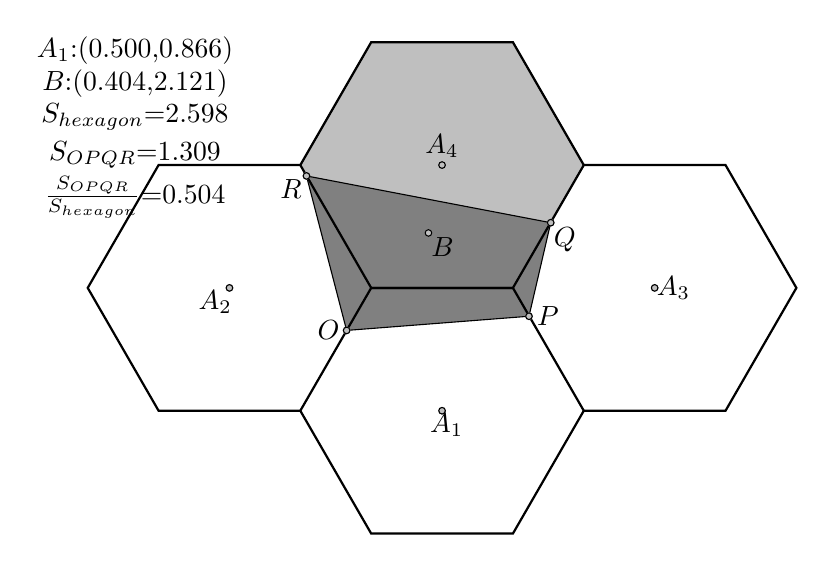
\begin{tikzpicture}[scale=0.6]
	
	\draw[black][fill=lightgray](4.5,7.8)--(3,10.4)--(0,10.4)--
	(-1.5,7.8)--(0,5.2)--(3,5.2)--cycle;
	
	\draw[black][fill=gray](-0.52,4.3) --(3.34,4.6)--(3.8,6.58)
	--(-1.37,7.57)--cycle;
	
	
	\draw[thick][black](0,0)--(3,0)--(4.5,2.6)--(7.5,2.6)--(9,5.2)
	--(7.5,7.8)--(4.5,7.8)--(3,10.4)--(0,10.4)--(-1.5,7.8)
	--(-4.5,7.8)--(-6,5.2)--(-4.5,2.6)--(-1.5,2.6)--cycle ;
	\draw[thick][black](4.5,2.6)--(3,5.2)--(0,5.2)--(-1.5,7.8) ;
	\draw[thick][black](-1.5,2.6)--(0,5.2)--(3,5.2)--(4.5,7.8) ;
	
	\draw[fill][lightgray](1.5,2.6) circle [radius=0.07];
	\draw(1.5,2.6) circle [radius=0.07];
	\node at (1.6,2.3){$A_1$};
	\draw[fill][lightgray](1.212,6.363) circle [radius=0.07];
	\draw(1.212,6.363) circle [radius=0.07];
	\node at (1.512,6.063){$B$};
	\draw[fill][lightgray](-3,5.2) circle [radius=0.07];
	\draw(-3,5.2) circle [radius=0.07];
	\node at (-3.3,4.9){$A_2$};
	\draw[fill][lightgray](6,5.2) circle [radius=0.07];
	\draw(6,5.2) circle [radius=0.07];
	\node at (6.4,5.2){$A_3$};
	\draw[fill][lightgray](1.5,7.8) circle [radius=0.07];
	\draw(1.5,7.8) circle [radius=0.07];
	\node at (1.5,8.2){$A_4$};
	
	\draw[fill][lightgray](-0.52,4.3) circle [radius=0.07];
	\draw(-0.52,4.3) circle [radius=0.07];
	\node at (-0.9,4.3){$O$};
	\draw[fill][lightgray](3.34,4.6) circle [radius=0.07];
	\draw(3.34,4.6) circle [radius=0.07];
	\node at (3.74,4.6){$P$};
	\draw[fill][lightgray](3.8,6.58) circle [radius=0.07];
	\draw(3.8,6.58) circle [radius=0.07];
	\node at (4.1,6.22){$Q$};
	\draw[fill][lightgray](-1.37,7.57) circle [radius=0.07];
	\draw(-1.37,7.57) circle [radius=0.07];
	\node at (-1.7,7.3){$R$};
	
	\node at (-5,10.22){$A_1$:(0.500,0.866)};
	\node at (-5,9.52){$B$:(0.404,2.121)};
	\node at (-5,8.82){$S_{hexagon}$=2.598};
	\node at (-5,8.02){$S_{OPQR}$=1.309};
	\node at (-5,7.12){$\frac{S_{OPQR}}{S_{hexagon}}$=0.504};
	\end{tikzpicture}	
\end{center}

We can choose a $B:(0.404,2.121)$ such that it changes more than half a 
hexagon, so this situation is also not good. \newline

We have finished all the theorems and given out some conclusions about 
this question. But it's a pity that we haven't solved the problem completely, 
we will give out some ideas about the question in next section